\documentclass[11pt,letter]{ivoa}
%\documentclass[11pt,letter]{ivoatex/ivoa}
%\input tthdefs
\input ivoatex/tthdefs

\newcommand{\xtype}[1]{\texttt{#1}}

\usepackage{longtable}
\usepackage{listings}
\lstloadlanguages{XML,sh}
\lstset{flexiblecolumns=true,basicstyle=\small,tagstyle=\ttfamily}
\usepackage[utf8]{inputenc}
\usepackage{todonotes}
\usepackage{enumerate}
\usepackage[section]{placeins}

\title{IVOA Architecture}

\ivoagroup{Technical Coordination Group}

\author{Janet Evans}
\author{Marco Molinaro}
\author{Patrick Dowler}
\author{Christophe Arviset}
\author{Severin Gaudet}
\author{IVOA Technical Coordination Group}

\editor{Janet Evans, Marco Molinaro}

\previousversion{IVOAArchitecture-2.0-20211029}
\previousversion{IVOAArchitecture-1.0-20101123}


\begin{document}

\begin{abstract}
This note describes the technical architecture of the International
Virtual Observatory Alliance
(IVOA). The description is decomposed 
into three levels. Level 0 is a general, high level summary of the IVOA
Architecture.
Level 1 provides more details about components and functionalities,
still without
being overly technical. Finally, Level 2 displays how the IVOA standards
fit into
the IVOA Architecture. This architecture enables the community of
resource providers to
implement the FAIR principles: Findable, Accessible, Interoperable, and
Reusable.
\end{abstract}

\section*{Acknowledgments}

\section{IVOA Architecture Level 0}

\begin{figure}[h]
\centering
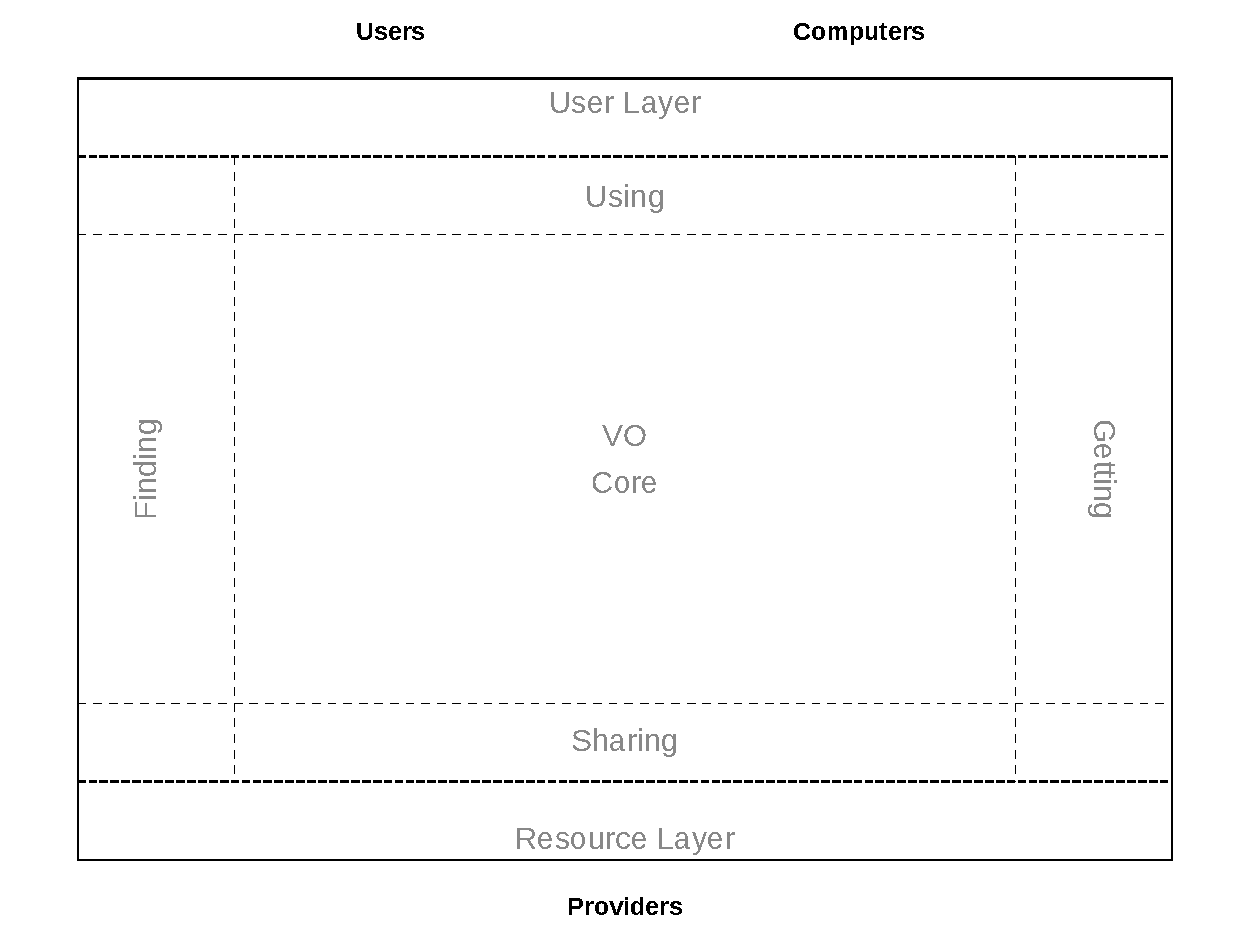
\includegraphics[width=0.9\textwidth]{archdiag0.pdf}
\caption{IVOA Architecture Level 0}
\label{fig:architecture0}
\end{figure}

Astronomy produces large amounts of data of many kinds, coming from
various sources:
science space missions, ground based telescopes, theoretical models,
compilation of
results, etc. These data are usually managed by large data centres or
smaller teams
and they provide the scientific community with data and/or computing
services
through the Internet. This is the Resource Layer. 

The ``consumers'' of these data and computing services, be it individual
researchers,
research teams or computer systems, interact with the User Layer. 

The Virtual Observatory (VO) is the necessary ``middle layer'' framework
connecting the
Resource Layer to the User Layer in a seamless and transparent manner.
Like the web
which enables end  users and machines to access documents and services 
wherever and however they are stored, the VO enables the astronomical
scientific
community to access astronomical resources wherever and however they are
stored by
the astronomical data and services providers. The VO provides a
technical framework
for the providers to enable users to discover data collections and
services
(``Findable'') and to use them for science and public outreach
(``Accessible''). To
enable these functionalities in perpetuity, it defines some core
astronomically-oriented
standards so data from different providers can be combined
(``Interoperable'') to enable
new scientific discoveries (``Reusable'').

The IVOA Architecture uses terms ``Finding'', ``Getting'', ``Using'',
and ``Sharing``;
these are collectively equivalent to ``Findable'', ``Accessible'',
``Interoperable'', and
``Reusable'': the FAIR principles have always been the basis of the IVOA
Architecture
even before the term was formally coined \citep{Wilkinson2016}. The
world wide
astronomy community has long supported sharing and reusability of data
(e.g. through standards
like FITS \citep{std:FITS}). Within the IVOA community, interoperability
has been the cornerstone
of development of standards and the concepts of reusability and
interoperability go beyond
metadata and data as they also guide the development of standards for
applications, services,
and infrastructure for research, education, and public outreach.

\section{IVOA Architecture Level 1}

Level 1 of the IVOA architecture is an extension to the Level 0,
displaying more
details about the functionalities and building blocks within the
different layers.
For completeness, part of the description is repeated from the Level 0,
so the
Level 1 description can be used as a self-contained block.

\begin{figure}[ht]
\centering
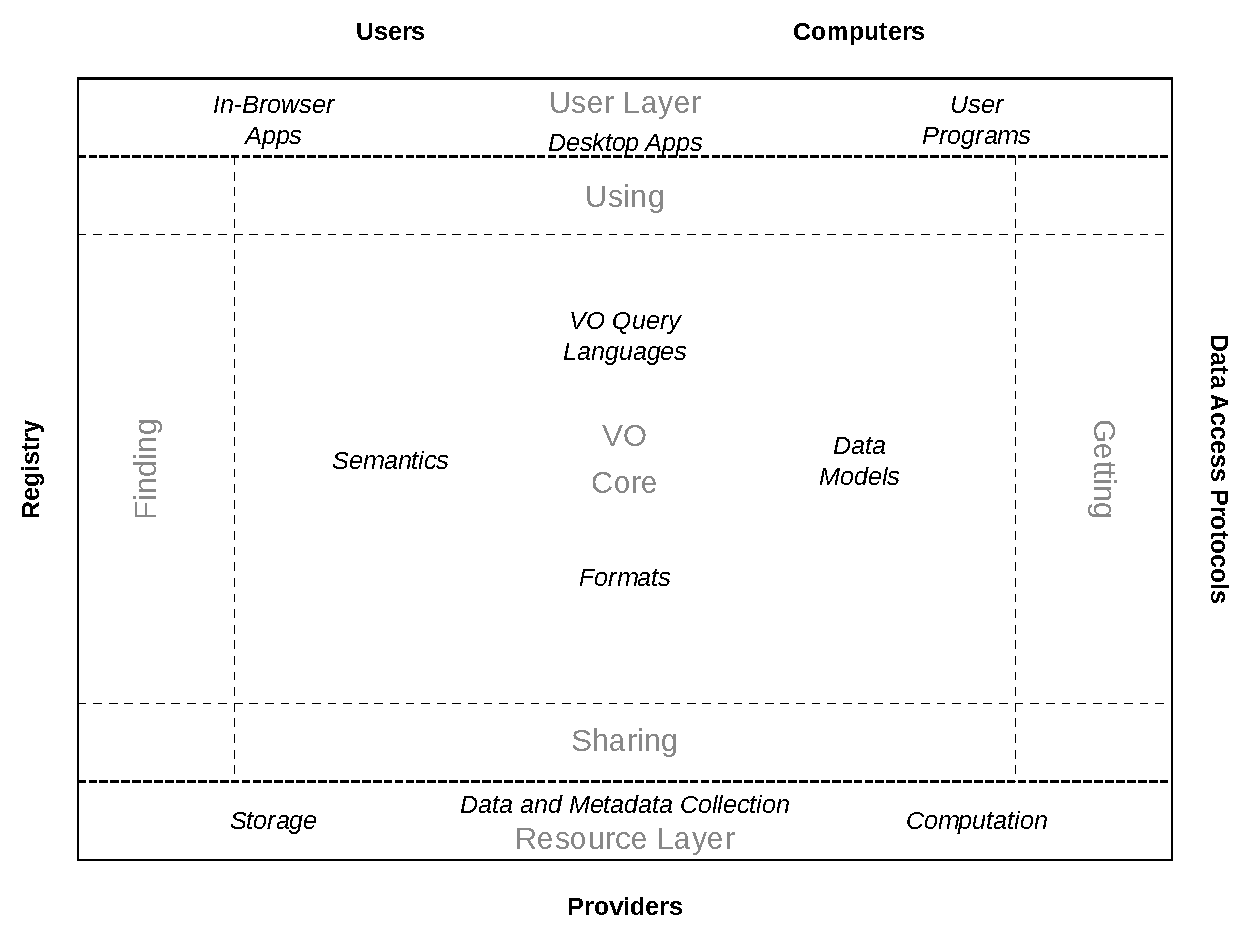
\includegraphics[width=0.9\textwidth]{archdiag1.pdf}
\caption{IVOA Architecture Level 1}
\label{fig:architecture1}
\end{figure}

Astronomy produces large amounts of data of many kinds, coming from
various sources:
science space missions, ground based telescopes, theoretical models,
compilation
of results, etc. These data are usually managed by large data centres or
smaller teams. These providers provide the scientific community with
data and
computing services through the Internet. These resources provided can
be:

\begin{enumerate}
\item data collections (images, spectra, time series, theoretical
models, catalogues, etc.)
with their associated descriptive metadata and access services.  
\item storage services for users and for processing 
\item computing services to process data from data collections and from
users
\end{enumerate}

This is the Resource Layer. 

The ``consumers'' of these data and computing services, be it individual
researchers,
research teams or computer systems, interact with the User Layer of the
IVOA architecture.
These interactions can be through browser based applications in a
typical web browser,
standalone desktop applications or scriptable applications that can be
used in interactive
and batch mode by a computer. 

The Virtual Observatory is the necessary ``middle layer'' framework that
connects the
Resource Layer to the User Layer in a seamless and transparent manner.
Like the web
that enables end users and machines to access transparently documents
and services
wherever and however they are stored, the VO enables the astronomical
scientific community
to access astronomical resources wherever and however they are stored by
the astronomical
data and services providers. The VO provides a technical framework for
the providers and
the consumers to share their data and services (``Sharing''). Registries
function as the ``yellow
pages'' of the VO, collecting metadata about data resources and
information services into a
queryable database. Like the VO resources and services themselves, the
registry is also
distributed. Replicas exist around the network, both for redundancy and
for more specialized
collections. Access to data and metadata collections is available
through Data Access Protocols,
which specify a uniform way of getting data and metadata from various
different providers.
To allow these functionalities, the definition of some core
astronomically-oriented standards
(``VO Core'') is necessary. In particular, defining common formats and
data models and using
common semantics is required to have a uniform and common description of
astronomical datasets
so they can become interoperable and queryable through standard query
languages to enable cross
analysis amongst various datasets. Additional standards are required
within the User Layer to enable
user authentication to proprietary datasets and storage elements as well
as interoperability amongst
VO applications (``Using'').

\section{IVOA Architecture Level 2}

Level 2 of the IVOA Architecture is similar to the Level 1, but adds all
the IVOA
standards in their corresponding layer. Some standards have already been
approved
and recommended (blue boxes with an outer line) while others are still a
work in progress
(blue boxes without an outer line).

\begin{figure}[ht]
\centering
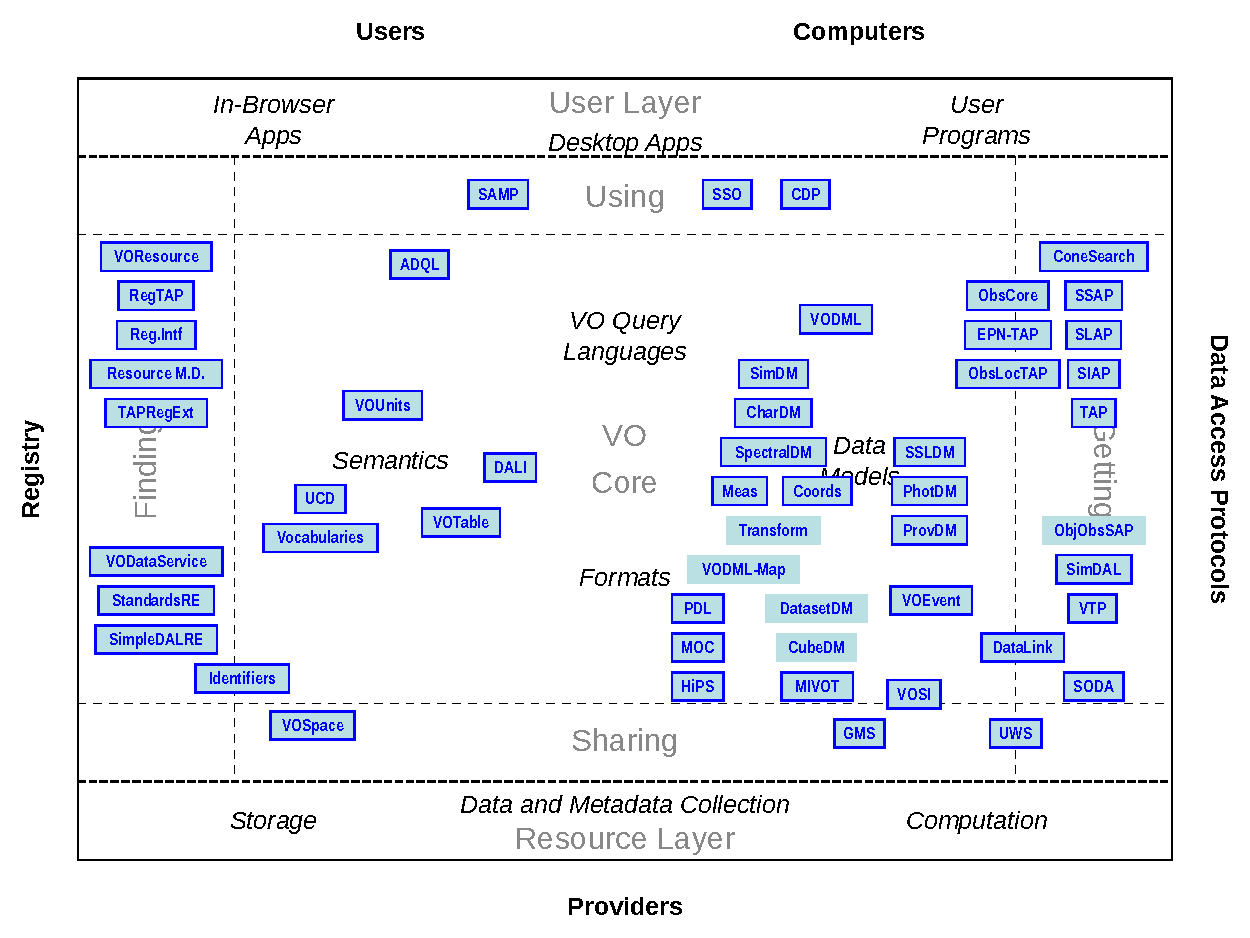
\includegraphics[width=0.9\textwidth]{archdiag2.pdf}
\caption{IVOA Architecture Level 2}
\label{fig:architecture2}
\end{figure}

Note that this list (and standard status) will naturally evolve with
time. Driven by
science use cases and implementation experience, existing standards will
be updated and
new standards will be identified and added to that
Fig.~\ref{fig:architecture2}.

The following sections of this document provide a summary description of
each current standard,
including a description of where it fits in the overall IVOA
architecture along with links with
other IVOA standards. The links 
(arrows) in the diagrams below indicate a ``used by'' dependency:
readers wanting to
understand the full scope of a standard will also need to review the
other standards
represented in each box of the diagrams. 
The standards shown in blue boxes are the subject of the section; 
boxes in light gray can be found in a different section/diagram. 
In some cases, green boxes are used to show external standards that
provide an
important or notable part of the IVOA standard. 
A white rounded box around several standards indicates a group of
standards that share
dependencies (to simplify the diagrams).

\section{Authentication and Authorization}

Authentication is a process by which you verify that someone is who they
claim they
are. Authorization is the process of establishing if the user (who is
already authenticated),
is permitted to have access to a resource. The authentication and
authorization architecture
is primarily an endorsement of existing
industry standards and technologies that suit the use cases of the IVOA
community. The standards
in this area provide some recommendations and ``glue'' so that
participants (application
developers, metadata and data providers, and resource providers) can
easily implement interoperable
systems.

Authentication and authorization are generally orthogonal to other
standards and there are minimal
direct dependencies on them. Implementors of other standards (e.g.
Sec.~\ref{dal} and \ref{gws})
``combine'' these A \& A recommendations where necessary to support
local policies and requirements.

\begin{figure}[ht]
\centering
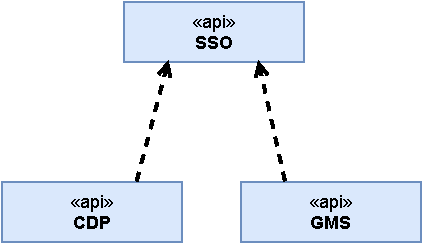
\includegraphics[width=0.28\textwidth]{ivoa-arch-auth.pdf}
\caption{Authentication and Authorization Standards and Dependencies}
\label{fig:authdeps}
\end{figure}

\subsection{SSO}

The Single-Sign-On (SSO) \citep{2017ivoa.spec.0524T} profile describes
authentication mechanisms. Approved client-server
authentication mechanisms are described for the IVOA single-sign-on
profile: No Authentication;
HTTP Basic Authentication; TLS with passwords; TLS with client
certificates; Cookies; Open
Authentication; Security Assertion Markup Language; OpenID. Normative
rules are given for
the implementation of these mechanisms, mainly by reference to
pre-existing standards.

\subsection{CDP}

The Credential Delegation Protocol (CDP) \citep{2010ivoa.spec.0218P}
allows a client program to delegate a user's credentials
to a service such that that service may make requests of other services
in the name of that
user. The protocol defines a REST service that works alongside other IVO
services to enable
such a delegation in a secure manner. In addition to defining the
specifics of the service
protocol, the standard document describes how a delegation service is
registered in an IVOA registry
along with the services it supports. The specification also explains how
one can determine
from a service registration that it requires the use of a supporting
delegation service.

\subsection{GMS}

The Group Membership Service (GMS) \citep{2022ivoa.spec.0222M}
specification describes a service interface for determining 
whether a user is a member of a group. Membership information can be
used to protect access to
proprietary resources. When an authorization decision is needed (whether
to grant or deny access
to a proprietary resource), a call to GMS can be made to see if the
requesting user is a member
of the group assigned to protect the resource in question. Examples of
proprietary resources are
wide ranging but include: observation data and metadata and scarce or
limited services and
infrastructure. Because this specification details how a single group
can protect multiple,
potentially distributed, resources, it allows for the representation of
teams with common
authorization rights. The members of such teams can span multiple
organizations but can be
managed within a single service. In this way, GMS offers an
interoperable, flexible, and
scalable mechanism for sharing proprietary assets with a potentially
dynamic set of team members.

\section{Application and Format Standards}

Application and Format Standards are focused on standards that support
data formats and
protocols that enable astronomy software tools to interoperate and
communicate. IVOA
members have recognised that building a monolithic tool that attempts to
fulfil all the
requirements of all users is impractical, and it is a better use of our
limited resources
to enable individual tools to work together better. One element of this
is defining
common file formats for the exchange of data between different
applications. Another
important component is a messaging system that enables the applications
to share data
and take advantage of each other's functionality.

\begin{figure}[ht]
\centering
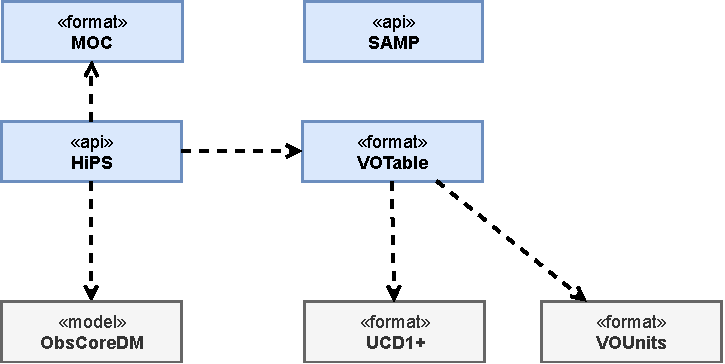
\includegraphics[width=0.48\textwidth]{ivoa-arch-apps.pdf}
\caption{Application and Format Standards and Dependencies}
\label{fig:appsdeps}
\end{figure}

\subsection{HiPS}

Hierarchical Progressive Survey (HiPS) \citep{2017ivoa.spec.0519F} is a
hierarchical scheme for the description, storage and
access of sky survey data. The system is based on hierarchical tiling of
sky regions at
finer and finer spatial resolution which facilitates a progressive view
of a survey, and
supports multi-resolution zooming and panning. HiPS uses the HEALPix
tessellation of the
sky as the basis for the scheme and is implemented as a simple file
structure with a direct
indexing scheme that leads to practical implementations. 

\subsection{MOC}

The Multi-Order Coverage Map (MOC) \citep{2022ivoa.spec.0727F} is a
method to specify coverage as an arbitrary sky regions.
The goal is to be able to provide a very fast comparison mechanism
between coverage maps.
The mechanism is based on the HEALPix sky tessellation algorithm. It is
essentially a
simple way to map regions of the sky into hierarchically grouped
predefined cells.

\subsection{VOTable} 

The VOTable \citep{2019ivoa.spec.1021O} format is an XML standard for
the interchange of data represented as a set of tables.
In this context, a table is an unordered set of rows, each of a uniform
structure, as specified
in the table description (the table metadata). Each row in a table is a
sequence of table cells,
and each of these contains either a primitive data type, or an array of
such primitives. VOTable
is derived from the Astrores format \citep{astrores}, itself modelled on
the FITS Table format
\citep{std:FITS}; VOTable was designed to be close to the FITS Binary
Table format.

\subsection{SAMP}

The Simple Application Messaging Protocol (SAMP)
\citep{2009ivoa.spec.1216B} is a messaging protocol that enables
astronomy
software tools to interoperate and communicate. SAMP supports
communication between
applications on the desktop and in web browsers, and is also intended to
form a framework
for more general messaging requirements. 

\section{Semantics Standards}

An interoperable data infrastructure needs common languages in many
places: From common designations of units to labels for physical
quantities, from common names of reference frames and time scales to
mutually understandable subject categories, from relationship types
between VO resources (``this service publishes images from A and spectra from B'') to fixed names for the messengers that produced the signals
recorded.

The VO's semantics standards provide the basis of forming such
consensual ``vocabularies'', which are, at their root, sets of labeled
concepts (which in turn are sets of entities clients deal with).  We
also take care that, wherever possible, our vocabularies are
interoperable with the rest of the semantic web by adopting the W3C's
Resource Description Framework RDF.

The vocabularies themselves are usually introduced by standards that use them and are then maintained on the VO's repository of
vocabularies\footnote{\url{http://www.ivoa.net/rdf}}.  In some cases,
however, we go beyond RDF, usually because the labels have an intrinsic
syntax.  In these cases, the Semantics WG issues separate standards
defining how to build and interpret these labels.  Currently, this is
the case for unit strings and for the Unified Content Descriptors
discussed below.

\begin{figure}[ht]
\centering
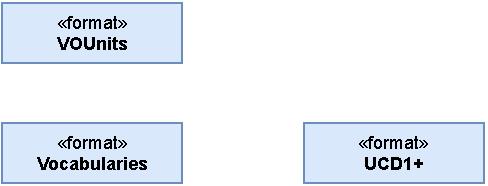
\includegraphics[width=0.32\textwidth]{ivoa-arch-semantics.pdf}
\caption{Semantics Standards and Dependencies}
\label{fig:semdeps}
\end{figure}

\subsection{Vocabularies}

Vocabularies in the VO \citep{2021ivoa.spec.0206D} describes how to
build and use
consensus vocabularies in the Virtual Observatory.  It supports both
``soft'' vocabularies based on the Simple Knowledge Organisation System
SKOS and ``hard'' vocabularies based on RDF schema, where the latter
organise their concepts in strict trees.  The ``hard'' vocabularies
enable simple inference with relatively little effort on the side of
the clients.  An example could be ``give me all links giving auxiliary
data for the current dataset'' in datalink, where vocabulary-aware
clients will also return links tagged as weight maps, errors, or noise
estimates.

This standard also details the maintenance of the VO's vocabulary
repository, in particular as regards adding vocabularies or concepts
within them.

\subsection{VOUnits}

VOUnits \citep{2023ivoa.spec.1215G} describes how to serialise unit
strings within the Virtual
Observatory, in particular (but by no means limited to) in the
\xmlel{unit} attribute in VOTable.  It hence defines the atomic units,
prefixes applicable, and the syntax of expressions using such prefixed
atomic units. 

An important design goal was consistency with other standards (BIPM,
ISO/IEC and the IAU) that are relevant in the astronomical community.
The intention is that units written to conform to VOUnits will likely
also be parsable by other well-known parsers.

\subsection{UCD}

Unified Content Descriptors (UCD) \citep{2019ivoa.spec.1007G} are a way
to
denote astronomical data
quantities.  The UCD formalism first defines a list of ``atoms'', in
effect a controlled vocabulary with a hierarchy implied through dots
(e.g., \ucd{pos} denotes positions, \ucd{pos.eq} equatorial positions);
this list is currently maintained as an Endorsed Note
\citep{2021ivoa.spec.0125C}.

The atoms can then be combined into more complex labels containing
qualifications.  For instance, \ucd{phot.mag;em.opt.V} denotes a
magnitude in the V band, \ucd{phot.flux;em.opt.V} a flux in the same
band.  The UCD standard defines how these compound UCDs are built, and
the UCD list defines restrictions as to where in complete UCDs atoms canbe used: some atoms can only be ``primary'', others are only available
as qualifiers.  For instance, \ucd{stat.error} can only appear at the
start of a UCD, which ensures that ``Error in redshift'' will be encoded as \ucd{stat.error;src.redshift} rather than the other way round.

The UCD ecosystem is completed by another standard on how new atoms are
adopted to the list of UCDs.

\section{Registry Standards}

The IVOA Registry provides a mechanism with which VO applications can
discover and select
resources that are relevant for a particular scientific problem. The VO
specification defines
the operation of this system. It is based on a general, distributed
model composed of searchable
and publishing registries. There are three components: (a) an interface
for harvesting publishing
registries, which builds upon the Open Archives Initiative Protocol for
Metadata Harvesting.
(b) A VOResource extension for registering registry services and
description of a central list
of said IVOA registry services. (c) A Registry of Registries as the root
component of data discovery
in the VO. 

\begin{figure}[ht]
\centering
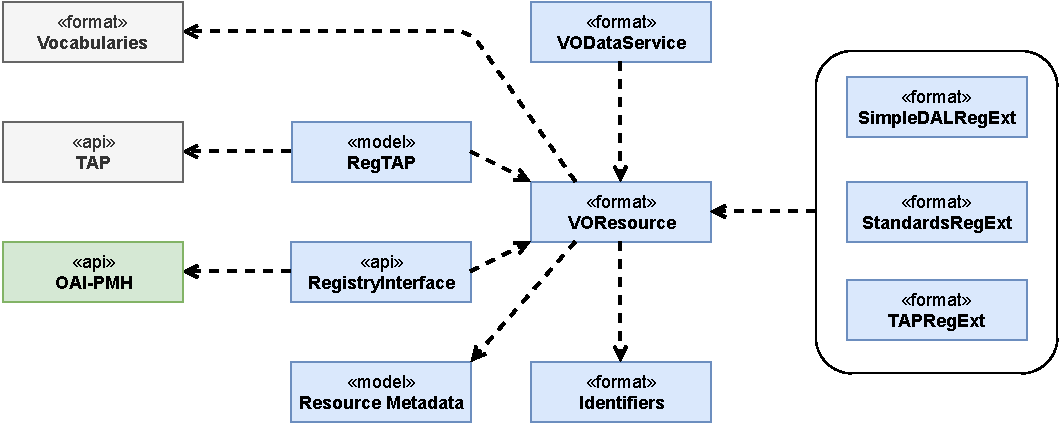
\includegraphics[width=0.70\textwidth]{ivoa-arch-registry.pdf}
\caption{Registry Standards and Dependencies}
\label{fig:regdeps}
\end{figure}

There are a number of standards associated with the registry to enable
registration and discovery
of services in the Registry. Figure \ref{fig:regdeps} shows how various
Registry standards relate to each other.

\subsection{Identifier}

An IVOA Resource Identifier (or IVOA identifier or IVOA ID for short)
\citep{2016ivoa.spec.0523D} is a globally unique reference
to a resource represented in a compact, ASCII-text format. An IVOA
identifier MUST always refer to
a resource that has been registered with an IVOA-compliant registry;
that is, it should be possible
to use the ID to get a description of the resource from a compliant
registry somewhere in the VO
environment.

\subsection{VOResource}

VOResource \citep{2018ivoa.spec.0625P} describes an encoding standard
for IVOA Resource Metadata. The primary intended use of
VOResource is to provide an XML interchange format for use with resource
registries. A registry is
a repository of resource descriptions and is employed by users and
applications to discover resources.
VOResource can be used to pass descriptions from publishers to
registries and then from registries to
applications. Another intended use is as a language for services to
describe themselves directly.

\subsection{VODataService}

The VODataService \citep{2021ivoa.spec.1102D} standard makes discovery
possible. It is an encoding standard that enables one to
describe how the data underlying the resource covers the sky as well as
their frequency and time.
VODataService also enables detailed descriptions of tables that include
information useful to the
discovery of tabular data. 

\subsection{Registry Interface}

The Registry Interface \citep{2018ivoa.spec.0723D} defines the
interfaces that support interactions between applications and
registries as well as between the registries themselves. It is based on
a general, distributed
model composed of searchable and publishing registries. The
specification has two main components:
(a) an interface for searching and (b) an interface for harvesting.
Finally, the Registry Interface
details the metadata used to describe registries themselves as resources
using an extension of the
VOResource metadata schema.

\subsection{Resource Metadata}

The Resource Metadata \citep{2007ivoa.spec.0302H} standard represents
the essential capability to describe what data and
computational facilities are available where, and once identified, how
to use them. The data
themselves have associated metadata (e.g., FITS keywords), and similarly
we require metadata
about data collections and data services so that VO users can easily
find information of interest.

\subsection{RegTAP}

The Registry Relational Schema for Table Access Protocol (RegTAP)
\citep{2019ivoa.spec.1011D} provides a mechanism
with which VO applications can discover and select resources - first and
foremost data and services
- that are relevant for a particular scientific problem. This
specification defines an interface
for searching this resource metadata based on the IVOA's TAP protocol.
It specifies a set of tables
that comprise a useful subset of the information contained in the
registry records, as well as the
table's data content in terms of the XML VOResource data model. The
general design of the system
is geared towards allowing easy authoring of queries. 

\subsection{SimpleDALRegExt}

Describing Simple Data Access Services (SimpleDALRegExt)
\citep{2022ivoa.spec.0222D}
is part of the registry standards that make discovery of Simple DAL
services
possible (e.g., SIAP, SCS, SSAP, SLAP). SimpleDALRegExt refers to an
encoding standard for a
specialized extension of the IVOA Resource Metadata that is useful for
describing VO Simple DAL
Services. By registering a VO Application in a Registry, it gets a
unique IVOA Resource
Identifier which then can be referred to by other applications and
services.

\subsection{StandardsRegExt}

The Standards registry extension (StandardsRegExt)
\citep{2012ivoa.spec.0508H} is part of the registry standards that make
discovery of VO Standards possible.
StandardsRegExt refers to an encoding standard for a specialized
extension of the IVOA Resource
Metadata that is useful for describing a VO Standard. By registering an
IVOA Standard in a
Registry, it gets a unique IVOA Resource Identifier which then can be
referred to in other
resource descriptions, namely for services that support the standard.

\subsection{TAPRegExt}

The Table Access Protocol registry extension (TAPRegExt)
\citep{2012ivoa.spec.0827D} is part of the registry standards that make
discovery of VO TAP Services possible.
TAPRegExt refers to an encoding standard for a specialized extension of
the IVOA Resource Metadata
that is useful for describing VO Applications. By registering a VO TAP
Service in a Registry, it
gets a unique IVOA Resource Identifier which then can be referred to by
other applications and
services. In the context of registering TAP services, an important role
filled by TAPRegExt is
the communication of supported data models to the registry.

\section{Data Model Standards}

The key element for achieving interoperability among actors sharing data
is the definition
of shared standard data models. Shared data models enable rich and
robust information sharing
between heterogeneous providers and users through a standard structure,
semantics, and formats;
data models are the foundation for this exchange.

\begin{figure}[ht]
\centering
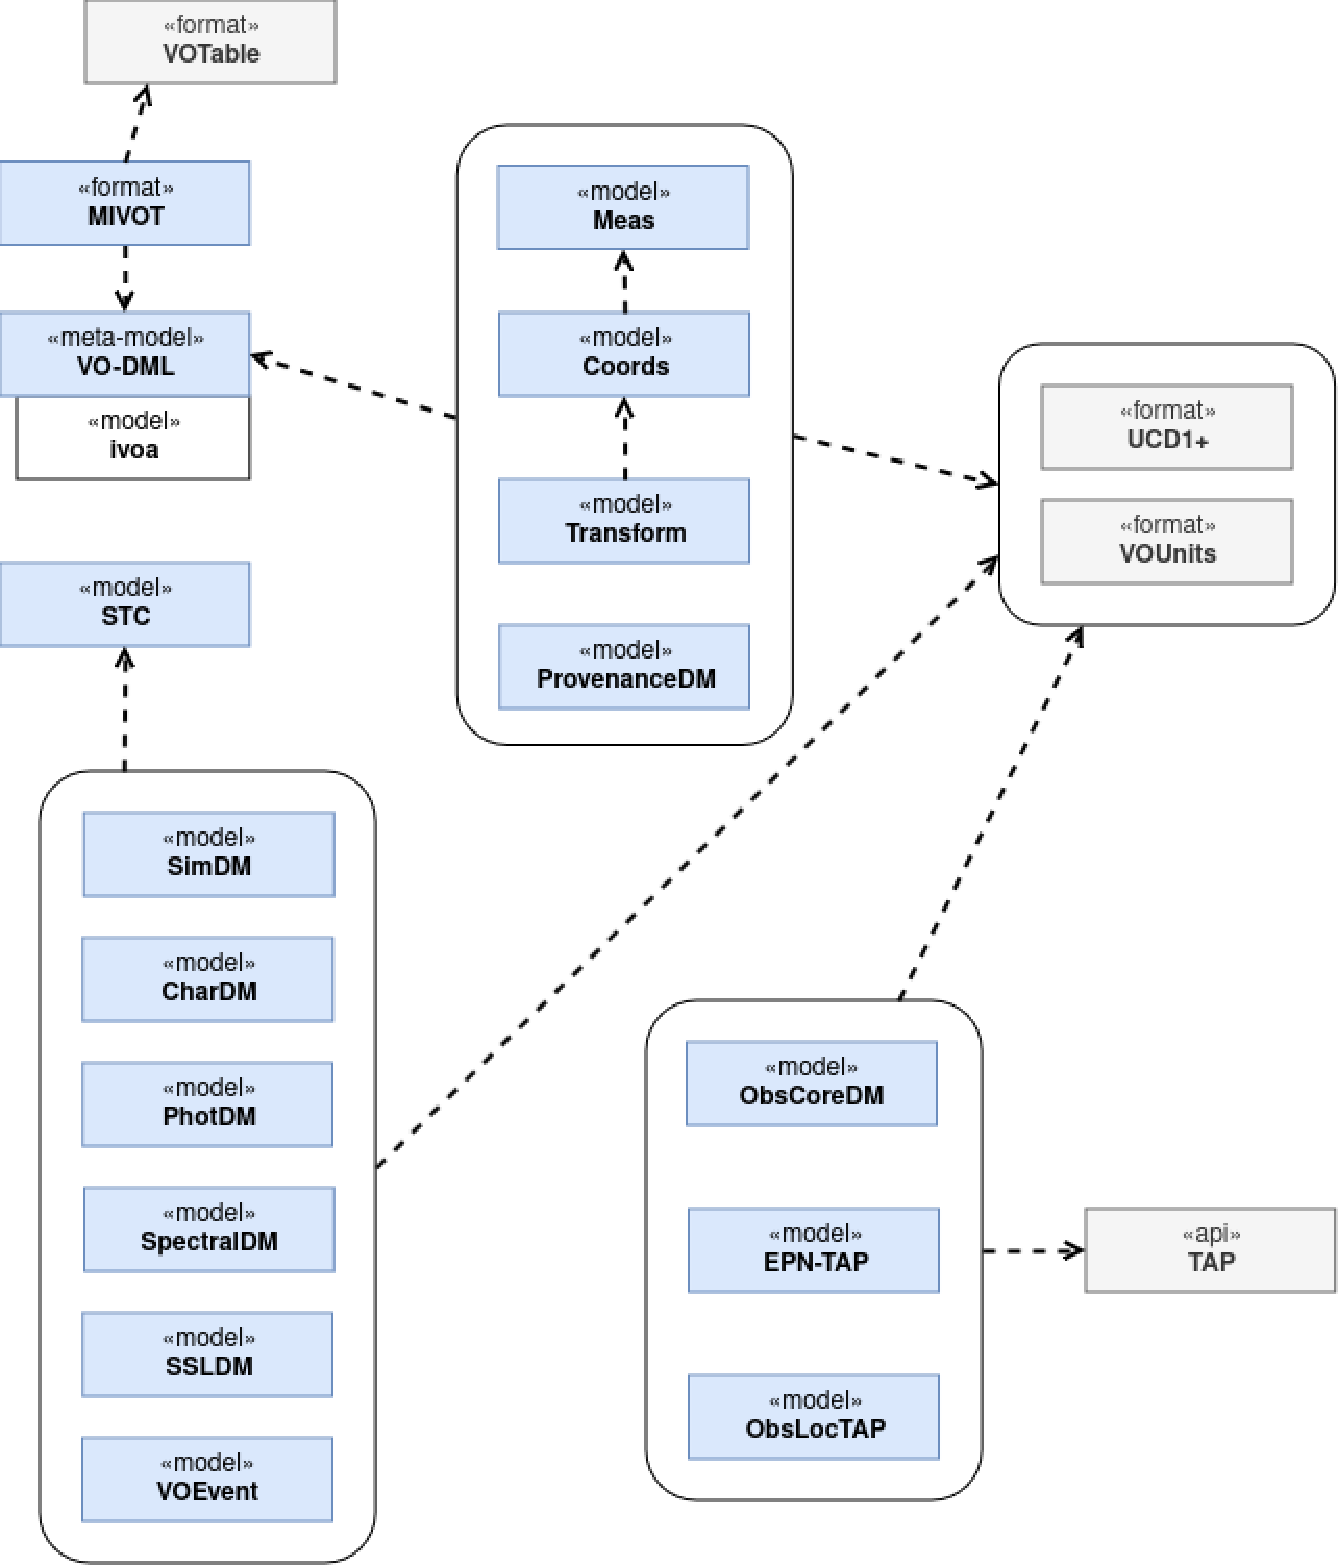
\includegraphics[width=0.62\textwidth]{ivoa-arch-dm.pdf}
\caption{Data Model Standards and Dependencies}
\label{fig:dmdeps}
\end{figure}

\subsection{VO-DML}

The VO Data Modelling Language (VO-DML) \citep{2018ivoa.spec.0910L}
defines a standard modelling language, or meta-model, for
expressing data models in the IVOA. Adopting such a uniform language for
all models allows
these to be used in a homogeneous manner and allows a consistent
definition of reuse of one
model by another. The particular language defined here includes a
consistent identification
mechanism for model which allows these to be referenced in an explicit
and uniform manner
also from other contexts, in particular from other IVOA standard formats
such as VOTable.
The language defined in this specification is named VO-DML (VO Data
Modelling Language).
VO-DML is a conceptual modelling language that is agnostic of
serializations, or physical
representations. This allows it to be designed to fit as many purposes
as possible. VO-DML
is directly based on UML, and can be seen as a particular representation
of a UML2 Profile.
VO-DML is restricted to describing static data structures and from UML
it only uses a subset
of the elements defined in its language for describing ``Class
Diagrams''. Its concepts can
be easily mapped to equivalent data modelling concepts in other
representations such as
relational databases, XML schemas and object-oriented computer
languages. VO-DML has a
representation as a simple XML dialect named VO-DML/XML that must be
used to provide the
formal representation of VO data models. VO-DML/XML aims to be concise,
explicit and
easy to parse and use in code that needs to interpret annotated data
sets. VO-DML as
described in this document is an example of a domain specific modelling
language, where the
domain here is defined as the set of data and meta-data structures
handled in the IVOA and
Astronomy at large. VO-DML provides a custom representation of such a
language and as a
side effect allows the creation and use of standards compliant data
models outside of the
IVOA standards context. 

\subsection{MIVOT} 

The Model Instances in VOTables (MIVOT) \citep{2023ivoa.spec.0620M}
defines a syntax to map VOTable data to any model serialized in VO-DML.
The annotation operates as a bridge between the data and the model. It
associates the column/param metadata from the VOTable to the data model
elements (class, attributes, types, etc.) of a standardized IVOA data
model, expressed in the Virtual Observatory Data Modeling Language (here
after VO-DML). It also brings up VOTable data or metadata that were
possibly missing in the table metadata. The data model elements are
grouped in an independent annotation block complying with the MIVOT XML
syntax. This annotation block is added as an extra resource element at
the top of the VOTable result resource. The MIVOT syntax allows to
describe a data structure as a hierarchy of classes. It is also able to
represent relations and composition between them. It can also build up
data model objects by aggregating instances from different tables of the
VOTable. Missing metadata can also be provided using MIVOT, for instance
by completing coordinate system description, or by providing curation
tracing. The annotation block is made of re-usable bricks that
facilitate the development of tools on both client and server sides. The
adopted design does not alter the original VOTable content. The backward
compatibility is preserved thanks to the limited impact of the
annotations on legacy clients.


\subsection{CharDM} 

The Characterisation Data Model (CharDM) \citep{2008ivoa.spec.0325L}
defines the high level metadata necessary to describe the
physical parameter space of observed or simulated astronomical data
sets, such as 2D-images,
data cubes, X-ray event lists, and IFU data. This model is an
abstraction which can be used
to derive a structured description of any relevant data and thus to
facilitate its discovery
and scientific interpretation. The model aims at facilitating the
manipulation of heterogeneous
data in any VO framework or portal. A VO Characterisation instance can
include descriptions of
the data axes, the range of coordinates covered by the data, and details
of the data sampling
and resolution on each axis. These descriptions should be in terms of
physical variables,
independent of instrumental signatures as far as possible.

\subsection{ObsCoreDM}

The Observation Data Model Core Components (ObsCoreDM)
\citep{2017ivoa.spec.0509L} specifies the metadata that are necessary to
perform data
discovery when querying data centers for astronomical observations of
interest. It exposes
use-cases to be carried out, explains the model and provides guidelines
for its implementation
as a data access service based on the Table Access Protocol (TAP). It
aims at providing a
simple model easy to understand and to implement by data providers that
wish to publish their
data into the Virtual Observatory. This interface integrates data
modelling and data access
aspects in a single service named ObsTAP that will be referenced as such
in the IVOA
registries. The Observation Data Model Core Components (ObsCoreDM)
defines
the core components of queryable metadata required for global discovery
of observational data.
It is meant to allow a single query to be posed to TAP services at
multiple sites to perform
global data discovery without having to understand the details of the
services present at each
site. It defines a minimal set of basic metadata and thus allows a
reasonable cost of
implementation by data providers. As with most of the VO Data Models,
ObsCoreDM makes use of STC, Utypes,
VOUnits and UCDs. The ObsCoreDM can be serialized as a VOTable.
ObsCoreDM makes reference
to more complete data models such as Characterisation DM, Spectrum DM or
Simple Spectral Line
Data Model (SSLDM). The current specification on the contrary provides
guidelines for
implementing these concepts using the TAP protocol and answering ADQL
queries. It is
dedicated to global discovery.

\subsection{PhotDM}

The Photometry Data Model (PhotDM) \citep{2022ivoa.spec.1101S} describes
photometry filters, photometric systems, magnitude
systems, zero points and its interrelation with the other IVOA data
models through a
simple data model. Particular attention is given necessarily to optical
photometry where
specifications of magnitude systems and photometric zero points are
required to convert
photometric measurements into physical flux density units.

\subsection{ProvenanceDM}

The Provenance Data Model \citep{2020ivoa.spec.0411S} describes how
provenance information can be modelled, stored
and exchanged within the astronomical community in a standardized way.
We follow the
definition of provenance as proposed by the W3C, i.e. that ``provenance
is information
about entities, activities, and people involved in producing a piece of
data or thing,
which can be used to form assessments about its quality, reliability or
trustworthiness''.
Such provenance information in astronomy is important to enable any
scientist to trace
back the origin of a dataset (e.g. an image, spectrum, catalog or single
points in a
spectral energy distribution diagram or a light curve), a document (e.g.
an article, a
technical note) or a device (e.g. a camera, a telescope), learn about
the people and
organizations involved in a project and assess the reliability, quality
as well as the
usefulness of the dataset, document or device for her own scientific
work.

\subsection{SimDM}

The Simulation Data Model (SimDM) \citep{2012ivoa.spec.0503L} describes
numerical computer simulations of astrophysical systems.
The primary goal of this standard is to support discovery of simulations
by describing those
aspects of them that scientists might wish to query on, i.e. it is a
model for meta-data
describing simulations. This document does not propose a protocol for
using this model.
IVOA protocols are being developed and are supposed to use the model,
either in its original
form or in a form derived from the model proposed here, but more suited
to the particular protocol.

\subsection{SSLDM}

The Simple Spectral Lines Data Model (SSLDM) \citep{2010ivoa.spec.1209O}
describes spectral line transitions. The main objective of
the model is to integrate with and support the Simple Line Access
Protocol, with which it forms
a compact unit. This integration allows seamless access to Spectral Line
Transitions available
worldwide in the VO context. This model does not provide a complete
description of Atomic and
Molecular Physics, which scope is outside of this document. In the
astrophysical sense, a line
is considered as the result of a transition between two energy levels.
Under the basis of this
assumption, a whole set of objects and attributes have been derived to
define properly the
necessary information to describe lines appearing in astrophysical
contexts.

\subsection{SpectralDM}

The Spectral Data Model \citep{2023ivoa.spec.1215C} describes the
structure of spectrophotometric datasets with spectral and
temporal coordinates and associated metadata. This data model may be
used to represent spectra,
time series data, segments of SED (Spectral Energy Distributions) and
other spectral or temporal
associations. 

\subsection{VOEvent} 

The VOEvent model \citep{2006ivoa.spec.0711S} defines the content and
meaning of a standard information packet for
representing, transmitting, publishing and archiving information about a
transient celestial
event, with the implication that timely follow-up is of interest. The
objective is to motivate
the observation of targets-of-opportunity, to drive robotic telescopes,
to trigger archive
searches, and to alert the community. VOEvent is focused on the
reporting of photon events,
but events mediated by disparate phenomena such as neutrinos,
gravitational waves, and solar
or atmospheric particle bursts may also be reported.

Structured data is used, rather than natural language, so that automated
systems can effectively
interpret VOEvent packets. Each packet may contain zero or more of the
``who, what, where, when, how''
of a detected event, but in addition, may contain a hypothesis (a
``why'') regarding the nature of
the underlying physical cause of the event. Citations to previous
VOEvents may be used to place
each event in its correct context. Proper curation is encouraged
throughout each event's life
cycle from discovery through successive follow-ups. VOEvent packets gain
persistent identifiers
and are typically stored in databases reached via registries. VOEvent
packets may therefore
reference other packets in various ways. Packets are encouraged to be
small and to be processed
quickly. This standard does not define a transport layer or the design
of clients, repositories,
publishers or brokers; it does not cover policy issues such as who can
publish, who can build a
registry of events, who can subscribe to a particular registry, nor the
intellectual property issues.

\subsection{STC}

The Space-Time Coordinate (STC) \citep{2007ivoa.spec.1030R} metadata for
the Virtual Observatory describes the coordinate
axes of astronomical data. It details the various components, highlights
some implementation
considerations, presents a complete set of UML diagrams, and discusses
the relation between
STC and certain other parts of the Data Model. Two serializations are
discussed: XML (STC-X) and
ascii string (STC-S); the former is an integral part of the model.

\subsection{Coordinates}

The Coordinates Data Model \citep{2022ivoa.specQ1004R} 
covers the following concepts: description of single and
multi-dimensional
coordinate space and coordinates within that space, cordinate frames
providing metadata describing the
origin and orientation of the coordinate space, the definition of simple
domain-specific coordinate
types for the most common use cases, and description of the coordinate
systems domain space. This
model is a refactored subset of the original STC data model.

\subsection{Measurements}

The Measurements Data Model \citep{2022ivoa.spec.1004R} 
covers the description of measured or determined astronomical data 
to enable the association of the determined ``value'' with corresponding
errors. In this model,
the ``value'' is given by the various coordinate types of the
coordinates data model plus a
description of the error model. This model is a refactored subset of the
original STC data model.

\subsection{ObsLocTAP} 

The Observation Locator Table Access Protocol (ObsLocTAP)
\citep{2021ivoa.spec.0724S}
defines a data model for scheduled observations 
and a method to run queries over compliant data, using several Virtual
Observatory technologies.
The data model builds on the ObsCore data model, removing elements
associated with dataset
access that are not available during the planning phase. In this way,
this standard is focused
on access to metadata related to the planning of a certain observatory,
more than on access to
the scientific data products. Also, the data model will be focused on
discovery of planned
observations, which is very useful information for multi-wavelength
coordination observations,
re-planning information propagation, follow-up of Targets of Opportunity
alerts, preparation
of proposals, etc. As with ObsCore, a serialisation into a relational
table is defined, which
allows users to run complex queries using the IVOA Table Access
Protocol. The document also
prescribes how to register and discover ObsLocTAP services. 

\section{Data Access Standards}
\label{dal}

The data access standards define APIs for querying and accessing data
holdings.
These standards are primarily implemented by data providers so that the
community
can use agreed and shared tools to interact with the data holdings.

As shown in Fig.~\ref{fig:daldeps}, the interconnection of data
access standards is quite complicated, even without showing the general
VO landscape
dependencies. This is due to two main
factors: older standards not yet updated to rely on DALI
(Sec.~\ref{dal:dali})
and protocols providing \textit{simple access} (parametric query
solutions) to
\textit{relational tablesets} (also supported by TAP,
Sec.~\ref{dal:tap}).

Supporting the data access standards, we also have the following
standards and specific cases:
\begin{itemize}
\item ADQL: a SQL-based language to allow querying of relational
databases, including support for astronomy operations;
	\item VTP: a specific transport protocol to broadcast VOEvent
messages;
	\item SimDAL: a dedicated access protocol, using SimDM structure and
concepts to allow access to simulated data collections.
\end{itemize}

\begin{figure}[ht]
\centering
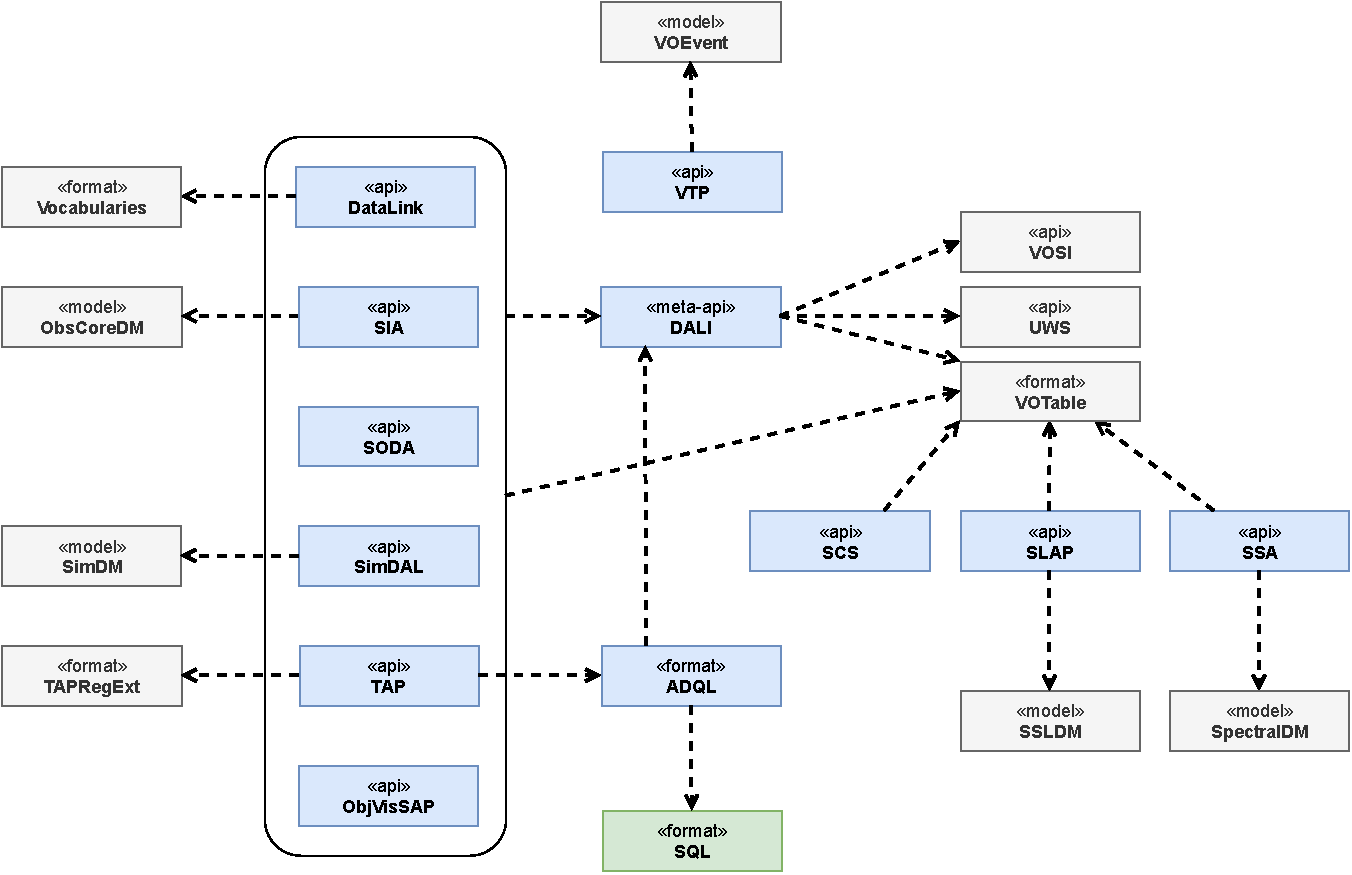
\includegraphics[width=0.90\textwidth]{ivoa-arch-dal.pdf}
\caption{Data Access Standards and Dependencies}
\label{fig:daldeps}
\end{figure}


\subsection{ADQL}

The Astronomical Data Query Language (ADQL) \citep{2023ivoa.spec.1215M}
has been developed based on SQL92. This document
describes the subset of the SQL grammar supported for querying
relational tablesets within the VO. Special restrictions and
extensions to SQL92 have been defined in order to support generic and
astronomy
specific operations. 

\subsection{ConeSearch}

The (simple) Cone Search (SCS) \citep{2008ivoa.specQ0222P} API
specification defines a simple query protocol for retrieving
records from a catalog of astronomical sources. The query describes sky
position and an
angular distance, defining a cone on the sky. The response returns a
list of astronomical
sources from the catalog whose positions lie within the cone, formatted
as a VOTable.

\subsection{DALI}
\label{dal:dali}

The Data Access Layer Interface (DALI) \citep{2017ivoa.spec.0517D}
defines the base web service interfaces common to all Data
Access Layer (DAL) services. This standard defines the behaviour of
common resources, the
meaning and use of common parameters, success and error responses, and
DAL service
registration. The goal of this specification is to define the common
elements that are
shared across DAL services in order to foster consistency across
concrete DAL service
specifications and to enable standard re-usable client and service
implementations and
libraries to be written and widely adopted. 

\subsection{DataLink}

The DataLink \citep{2023ivoa.spec.1215B} API specification describes the
linking of data discovery metadata to
the data itself, further detailed metadata, related resources, and to
services that perform
operations on the data. The web service capability supports a drill-down
into the details
of a specific dataset and provides a set of links to the dataset file(s)
and related resources.
This specification also includes a VOTable-specific method of providing
descriptions of one
or more services and their input(s), usually using parameter values from
elsewhere in the
VOTable document. Providers are able to describe services that are
relevant to the records
(usually datasets with identifiers) by including service descriptors in
a result document.

\subsection{SIA}

The Simple Image Access (SIA) \citep{2015ivoa.spec.1223D} protocol
provides capabilities for the discovery, description,
access, and retrieval of multi-dimensional image datasets, including 2-D
images as well
as datacubes of three or more dimensions. SIA data discovery is based on
the ObsCore Data
Model, which primarily describes data products by the physical axes
(spatial, spectral,
time, and polarization). Image datasets with dimension greater than 2
are often referred
to as datacubes, cube or image cube datasets and may be considered
examples of hypercube
or n-cube data. In this document the term ``image'' refers to general
multi-dimensional
datasets and is synonymous with these other terms unless the image
dimensionality is
otherwise specified. SIA provides capabilities for image discovery and
access. Data
discovery and metadata access (using ObsCoreDM) are defined here. The
capabilities for
drilling down to data files (and related resources) and services for
remote access are
defined elsewhere, but SIA also allows for direct access to retrieval. 

\subsection{SimDAL}

The Simulation Data Access Layer (SimDAL) \citep{2017ivoa.spec.0320L}
protocol defines a set of resources and associated
actions to discover and retrieve simulations and numerical models in the
Virtual Observatory.
SimDAL and the Simulation Data Model are dedicated to cover the needs
for the publication
and retrieval of any kind of simulations: N-body or MHD simulations,
numerical models of
astrophysical objects and processes, theoretical synthetic spectra,
etc... SimDAL is
divided in three parts. First, SimDAL Repositories store the
descriptions of theoretical
projects and numerical codes. They can be used by clients to discover
theoretical
services associated with projects of interest. Second, SimDAL Search
services are
dedicated to the discovery of precise datasets. Finally, SimDAL Data
Access services
are dedicated to retrieve the original simulation output data, as plain
raw data or
formatted datasets cut-outs. To manage any kind of data, eventually
large or at
high-dimensionality, the SimDAL standard lets publishers choose any
underlying
implementation technology. 

\subsection{SLAP}

The Simple Line Access Protocol (SLAP) \citep{2010ivoa.specQ1209O} is an
IVOA data access protocol which defines a protocol
for retrieving spectral lines coming from various Spectral Line Data
Collections through a
uniform interface within the VO framework. These lines can be either
observed or theoretical
and will be typically used to identify emission or absorption features
in astronomical
spectra. It makes use of the Simple Spectral Line Data Model to
characterize spectral lines
through the use of utypes. The SLAP interface is meant to be reasonably
simple to implement
by service providers. A basic query will be done in a wavelength range
for the different
services. The service returns a list of spectral lines formatted as a
VOTable. Thus, an
implementation of the service may support additional search parameters
(some which may be
custom to that particular service) to more finely control the selection
of spectral lines.
The specification also describes how the search on extra parameters has
to be done, making
use of the support provided by the Simple Spectral Line Data Model

\subsection{SSAP}

The Simple Spectral Access Protocol (SSAP) \citep{2012ivoa.spec.0210T}
defines a uniform interface to remotely discover and
access one dimensional spectra. SSA is a member of an integrated family
of data access
altogether comprising the Data Access Layer (DAL) of the IVOA. SSA is
based on a more
general data model capable of describing most tabular spectrophotometric
data, including
time series and spectral energy distributions (SEDs) as well as 1-D
spectra; however the
scope of the SSA interface as specified in this document is limited to
simple 1-D spectra,
including simple aggregations of 1-D spectra. The form of the SSA
interface is simple:
clients first query the global resource registry to find services of
interest and then
issue a data discovery query to selected services to determine what
relevant data is
available from each service; the candidate datasets available are
described uniformly
in a VOTable format document which is returned in response to the query.
Finally, the
client may retrieve selected datasets for analysis. Spectrum datasets
returned by an SSA
spectrum service may be either precomputed, archival datasets, or they
may be virtual
data which is computed on the fly to respond to a client request.
Spectrum datasets may
conform to a standard data model defined by SSA, or may be native
spectra with custom
project-defined content. Spectra may be returned in any of a number of
standard data
formats. Spectral data is generally stored externally to the VO in a
format specific to
each spectral data collection; currently there is no standard way to
represent astronomical
spectra, and virtually every project does it differently. Hence spectra
may be actively
mediated to the standard SSA-defined data model at access time by the
service, so that
client analysis programs do not have to be familiar with the
idiosyncratic details of each
data collection to be accessed. 

\subsection{SODA} 

The Server-side Operations for Data Access (SODA)
\citep{2017ivoa.spec.0517B} is an API for low-level data access or
server side
data processing. The initial version describes operations for extracting
a subsection of a data
file using astronomical coordinates; Future evolution is expected to
include performing
various kinds of operations: transformations, pixel operations, and
applying functions to the data.

\subsection{TAP}
\label{dal:tap}

The Table Access Protocol (TAP) \citep{2019ivoa.spec.0927D} defines a
service protocol for accessing general table data,
including astronomical catalogs as well as general database tables.
Access is provided
for both database and table metadata as well as for actual table data.
This version of
the protocol includes support for multiple query languages, including
queries specified
using the Astronomical Data Query Language within an integrated
interface. It also
includes support for both synchronous and asynchronous queries. Special
support is
provided for spatially indexed queries using the spatial extensions in
ADQL. A multi-position
query capability permits queries against an arbitrarily large list of
astronomical targets,
providing a simple spatial cross-matching capability. More sophisticated
distributed
cross-matching capabilities are possible by orchestrating a distributed
query across
multiple TAP services. 

\subsection{EPN-TAP}
\label{epn:tap}

The EPN-TAP protocol \citep{2022ivoa.spec.0822E} defines a service
protocol for describing and accessing data related to the study of the
Solar System in general, including observational, modeled, and
experimental data. It consists of 1) the usual TAP mechanism; 2) the
EPNcore metadata dictionary; 3) a set of rules defining table structure
and parameter usage. EPN-TAP relies on the TAP standard
({Sec.~\ref{epn:tap}) with no modification. All EPN-TAP services are
accessible through standard TAP clients.


\subsection{VTP}

The VOEvent Transport Protocol (VTP) \citep{2017ivoa.spec.0320S}
formalizes a TCP-based protocol for VOEvent transportation
that has been in use by members of the VOEvent community for several
years and discusses
the topology of the event distribution network. It is intended to act as
a reference for
the production of compliant protocol implementations. 

\section{Infrastructure Resource Standards}
\label{gws}

Infrastructure resource standards define or sanction APIs and formats to
support for access
to shared resources: computing, storage, and science platforms. These
standards borrow from
or sanction industry standards or provide a common abstraction for users
that can be implemented
on top of industry standard infrastructure.

\begin{figure}[ht]
\centering
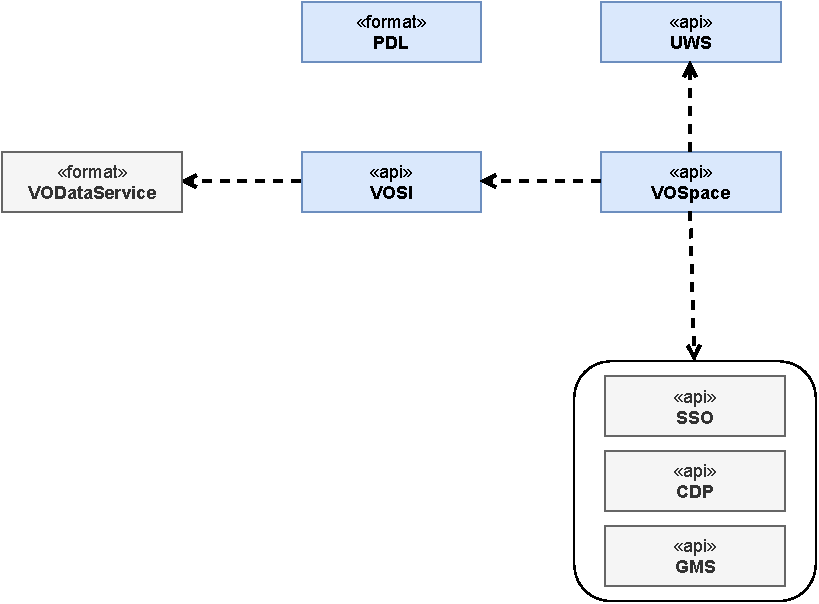
\includegraphics[width=0.54\textwidth]{ivoa-arch-gws.pdf}
\caption{Authentication and Authorization Standards and Dependencies}
\label{fig:gwsdeps}
\end{figure}

\subsection{PDL}

The Parameter Description Language (PDL) \citep{2014ivoa.spec.0523Z}
defines a language where parameters are described in a
rigorous data model. With no loss of generality, we will represent this
data model using
XML. It intends to be a expressive language for self-descriptive web
services exposing
the semantic nature of input and output parameters, as well as all
necessary complex
constraints. PDL is a step forward towards true web services
interoperability.
 
\subsection{UWS} 

The Universal Worker Service (UWS) \citep{2016ivoa.spec.1024H} pattern
defines how to manage asynchronous execution
of jobs on a service. Any application of the pattern defines a family of
related services
with a common service contract. Possible uses of the pattern are also
described.

\subsection{VOSI} 

This VO Service Interface (VOSI) \citep{2017ivoa.spec.0524G} describes
the minimum interface that a web service requires to
participate in the world-wide network of VO services. Note that this is
not required of
standard VO services developed prior to this specification, although
uptake is strongly
encouraged on any subsequent revision. All new standard VO services,
however, must feature
a VOSI-compliant interface. 

\subsection{VOSpace}

The VOSpace \citep{2018ivoa.spec.0621G} API defines an interface to
distributed storage. This specification presents the
second RESTful version of the interface. It specifies how VO agents and
applications can
use network attached data stores to persist and exchange data in a
standard way.

\pagebreak
\section{Acronym Lookup Table}

\begin{longtable}[t]{l l}
        \sptablerule
        \textbf{Acronym} & \textbf{Expansion} \\
        \sptablerule
        {ADQL} & 
        {Astronomical Data Query Language - standard} \\
        {API} & 
        {Application programming Interface} \\
        {CDP} &
        {Credential Delegation Protocol - standard} \\
        {CharDM} &
        {Characterisation Data Model - standard} \\
        {ConeSearch} &
        {Cone Search - simple positional search service standard} \\
        {Coords} &
        {Coordinates - astronomical coordinates standard} \\
        {DALI} &
        {Data Access Layer Interface - common components standard} \\
        {DataLink} &
        {Data Link - linking metadata to data standard} \\
       {EPN-TAP} &
       {Solar System Table access protocol} \\
        {GMS} &
        {Group Membership Service - standard} \\
        {HiPS} &
        {Hierarchical Progressive Survey - standard} \\
        {Identifier} &
        {Identifier standard for URI(s) with the ``ivo'' scheme} \\
        {IVOA} &
        {International Virtual Observatory Alliance} \\
        {Meas} &
        {Measurements - astronomical measurements standard} \\
        {MIVOT} &
        {MIVOT - model instances in VO tables} \\
        {MOC} &
        {Multi-Order Coverage - metadata standard} \\
        {ObsCoreDM} &
        {Observation Core Data Model - standard} \\
        {ObsLocTAP}  &
        {Observation Locator (relational model) for TAP - standard} \\
        {PDL} &
        {Parameter Description Language - standard} \\
        {PhotDM} &
        {Photometry Data Model - standard} \\
        {PR} &
{Proposed Recommendation - the "proposed" status for standards} \\        {ProvenanceDM} &
        {Provenance Data Model - standard} \\
        {REC} &
{Recommendation - the final "recommended" status for standards} \\        {Registry Interface} &
        {Registry Interface - standard} \\
        {RegTAP} &
        {Registry (relational model) for TAP - standard} \\
        {Resource Metadata} &
        {Resource Metadata - model/serialisation standard} \\
        {SAMP} &
        {Simple Application Messagign Protocol - stanadrd} \\
        {SIA} &
        {Simple Image Access - standard} \\
        {SIAP} &
        {Simple Image Access Protocol - see SIA}  \\
        {SimDAL} &
        {Simulation Data Access Layer - standard} \\
        {SimDM} &
        {Simulation Data Model - standard} \\
        {SimpleDALRegExt} &
        {Simple Data Access Layer Registry Extension - standard} \\
        {SLAP} &
        {Simple Line Access Protocol - standard} \\
        {SODA}  &
        {Server-side Operations for Data Access - standard} \\
        {SpectralDM} &
        {Spectral Data Model - standard} \\
        {SSAP} &
        {Simple Spectral Access Protocol - standard} \\
        {SSLDM} &
        {Simple Spectral Line Data Model - standard} \\
        {SSO} &
        {Single Sign On - standard} \\
        {StandardsRegExt} &
        {Standards Registry Extension - standard} \\
        {STC} &
        {Space Time Coordinates - standard} \\
        {TAP} &
        {Table Access Protocol - standard} \\
        {TAPRegExt} &
        {Table Access Protocol Registry Extension - standard} \\
        {UCD} &
        {Univeral Content Descriptor - standard} \\
        {URI}  &
        {Universal Resource Identifider - standard} \\
        {UWS}  &
        {Univeral Worker service - standard} \\
        {Vocabularies} &
        {Vocabularies standard for the IVOA} \\
        {VODataService} &
{Virtual Observatory Data Service service metadata - standard} \\        {VO-DML} &
        {Virtual Observatory Data Modelling Language - standard} \\
        {VOEvent}  &
        {Virtual Observatory Event - standard} \\
        {VOResource} &
        {Virtual Observatory Resource - metadata standard} \\
        {VOSI} &
{Virtual Observatory Support Interfaces - common components standard} \\        {VOSpace} &
        {Virtual Observatory Space - user storage standard} \\
        {VOTable} &
        {Virtual Observatory Table - standard} \\
        {VOUnits} &
        {Virtual Observatory Units - standard} \\
        {VTP} &
        {VOEvent Transport Protocol - standard} \\
        {WD} & 
        {Working Draft - early "draft" status for standards} \\
        \sptablerule
\end{longtable}


\bibliography{ivoatex/ivoabib,ivoatex/docrepo,localrefs}

\end{document}
